 
\documentclass[a4paper,12pt]{article} % This defines the style of your paper

\usepackage[top = 2.5cm, bottom = 2.5cm, left = 2.5cm, right = 2.5cm]{geometry}
\usepackage[T1]{fontenc}
\usepackage[utf8]{inputenc}
\usepackage{multirow} % Multirow is for tables with multiple rows within one cell.
\usepackage{booktabs} % For even nicer tables.
\usepackage{graphicx} 
\usepackage{setspace}
\setlength{\parindent}{0in}
\usepackage{float}
\usepackage{fancyhdr}

\usepackage{tikz}
\usepackage{pgfplots}
\usepgfplotslibrary{polar}

\usepackage{hyperref,graphicx,lmodern}
\usepackage{xcolor}
\usepackage{nicefrac}
\usepackage{upgreek}
\usepackage[]{bm}
\usepackage{amsmath}
\usepackage[]{mathtools}

\graphicspath{{imgs/}}

\usepackage[]{listings}

\definecolor{codegreen}{rgb}{0,0.6,0}
\definecolor{codegray}{rgb}{0.5,0.5,0.5}
\definecolor{codepurple}{rgb}{0.58,0,0.82}
\definecolor{backcolour}{rgb}{1.0, 1.0, 1.0}

\lstdefinestyle{mystyle}{
  backgroundcolor=\color{backcolour},
  commentstyle=\color{codegreen},
  keywordstyle=\color{magenta},
  numberstyle=\tiny\color{codegray},
  stringstyle=\color{codepurple},
  basicstyle=\ttfamily\footnotesize,
  breakatwhitespace=false,
  breaklines=true,
  captionpos=b,
  keepspaces=true,
  numbers=left,
  numbersep=5pt,
  showspaces=false,
  showstringspaces=false,
  showtabs=false,
  tabsize=2
}

\lstset{style=mystyle}


%%%%%%%%%%%%%%%%%%%%%%%%%%%%%%%%%%%%%%%%%%%%%%%%
% 3. Header (and Footer)
%%%%%%%%%%%%%%%%%%%%%%%%%%%%%%%%%%%%%%%%%%%%%%%%
\pagestyle{fancy} % With this command we can customize the header style.
\fancyhf{} % This makes sure we do not have other information in our header or footer.

\lhead{\footnotesize QM: Homework 1}% \lhead puts text in the top left corner. \footnotesize sets our font to a smaller size.

\rhead{\footnotesize Lastname 1, Lastname 2 (\& Lastname 3)} %<---- Fill in your lastnames.

\cfoot{\footnotesize \thepage}

\begin{document}


%%%%%%%%%%%%%%%%%%%%%%%%%%%%%%%%%%%%%%%%%%%%%%%%
%%%%%%%%%%%%%%%%%%%%%%%%%%%%%%%%%%%%%%%%%%%%%%%%

%%%%%%%%%%%%%%%%%%%%%%%%%%%%%%%%%%%%%%%%%%%%%%%%
% Title section of the document
%%%%%%%%%%%%%%%%%%%%%%%%%%%%%%%%%%%%%%%%%%%%%%%%

% For the title section we want to reproduce the title section of the Problem Set and add your names.

\thispagestyle{empty} % This command disables the header on the first page. 

\begin{tabular}{p{15.5cm}} % This is a simple tabular environment to align your text nicely 
{\large \bf Introduction au calcul scientifique} \\
Arts \& Métiers Sciences \& Technologies \\
Année universitaire : 2020-2021 \\
\hline % \hline produces horizontal lines.
\\
\end{tabular} % Our tabular environment ends here.

\vspace*{0.3cm} % Now we want to add some vertical space in between the line and our title.

\begin{center} % Everything within the center environment is centered.
	{\Large \bf Recherche de racines} % <---- Don't forget to put in the right number
	\vspace{2mm} % <---- Fill in your names here!
\end{center}  

\vspace{0.4cm}

%%%%%%%%%%%%%%%%%%%%%%%%%%%%%%%%%%%%%%%%%%%%%%%%
%%%%%%%%%%%%%%%%%%%%%%%%%%%%%%%%%%%%%%%%%%%%%%%%

L'objectif de cette séance de travaux pratiques est de vous familiariser avec les méthodes de recherche de racines.
Pour cela nous considérerons un problème classique d'artillerie~: déterminer l'angle de hausse $\theta$ d'un canon afin d'atteindre une cible pré-déterminée.
En partant des principes de Newton, on supposera que les équations du mouvement sont données par
%
\[
\begin{aligned}
  m \ddot{x} & = -k \dot{x} \\
  m \ddot{y} & = -k \dot{y} - mg
\end{aligned}
\]
%
où $m$ est la masse du projectile, $k$ le coefficient de friction avec l'air et $g$ est l'accélération gravitationelle à la surface de la Terre.
Ce jeu d'équations est supplémenté avec les conditions initiales suivantes :
%
\[
\begin{aligned}
  x(0) & = y(0) = 0 \\
  \dot{x}(0) & = v_0 \cos(\theta) \\
  \dot{y}(0) & = v_0 \sin(\theta)
\end{aligned}
\]
%
où $v_0$ est la vitesse d'éjection du canon.
L'objectif est alors de déterminer l'angle de hausse $\theta$ du canon de façon à toucher la cible située à une distance $D$ de l'artilleur.

\subsection*{Cas sans frottement}

Commençons par étudier le cas sans frottement (i.e.\ $k = 0$).
Les équations du mouvement se réduisent alors à
%
\[
\begin{aligned}
  \dot{x} & = v_0 \cos(\theta) \\
  \ddot{y} & = -g
\end{aligned}
\]
%
auxquelles on adjoint les conditions initiales
%
\[
\begin{aligned}
  x(0) & = y(0) = 0 \\
  \dot{y}(0) & = v_0 \sin(\theta).
\end{aligned}
\]

\begin{enumerate}
\item Montrez que les équations horaires du mouvement sont données par
  %
  \[
  \begin{aligned}
    x(t) & = v_0 \cos(\theta) t \\
    y(t) & = -\dfrac{1}{2} gt^2 + v_0\sin(\theta) t.
  \end{aligned}
  \]
  %
  En déduire que la trajectoire du mouvement est donnée par
  %
  \[
  y(x, \theta) = -\dfrac{1}{2} \dfrac{g}{v_0^2 \cos^2(\theta)} x^2 + \tan(\theta) x.
  \]
  %
  On rappelle que $\tan(\theta) = \nicefrac{\sin(\theta)}{\cos(\theta)}$.

\item Montrez que la distance parcourue par le projectile avant de toucher le sol est donnée par
  %
  \[
  D(\theta) = \dfrac{v_0^2}{g} \sin(2\theta)
  \]
  %
  où l'on utilise le fait que $\cos(\theta) \sin(\theta) = \sin(2\theta)$.
  Montrez que la portée maximale du canon est atteinte pour un angle de hausse $\theta = \nicefrac{\pi}{4}$.

\item En utilisant la fonction \verb+root_scalar+ du package \verb+scipy.optimize+, écrivez une fonction \verb+python+ prenant en entrée la vitesse d'éjection $v_0$ du canon et la distance $D$ à laquelle est située la cible et permettant de
  \begin{enumerate}
  \item vérifier que la cible est à portée du canon (i.e. $D \leq D_{\max}$),
  \item si oui, alors calculez l'angle de hausse $\theta$ nécessaire pour toucher la cible.
    Vous pouvez utiliser la méthode de votre choix (i.e. \verb+'bisect'+, \verb+'secant'+ ou \verb+'newton'+).
  \end{enumerate}

\item Utilisez votre code pour déterminer l'angle de hausse $\theta$ si les données d'entrée sont $v_0 = 10$, $g=10$ et $D = 5$.
\end{enumerate}

\subsection*{Cas avec frottement}

Intérressez nous maintenant au cas avec frottement (i.e.\ $k \neq 0$).
Les équations du mouvement sont alors données par
%
\[
\begin{aligned}
  \ddot{x} & = -\dfrac{k}{m} \dot{x} \\
  \ddot{y} & = -g - \dfrac{k}{m} \dot{y}
\end{aligned}
\]
%
auxquelles on adjoint les conditions initiales suivantes
%
\[
\begin{aligned}
  x(0) & = y(0) = 0 \\
  \dot{x}(0) & = v_0 \cos(\theta) \\
  \dot{y}(0) & = v_0 \sin(\theta).
\end{aligned}
\]
%
Afin de simplifier les calculs, on peut \textbf{adimensioner} les équations en introduisant les changements de variables suivants
%
\[
\begin{aligned}
  x & \to \dfrac{v_0^2}{g} x \\
  y & \to \dfrac{v_0^2}{g} y \\
  t & \to \dfrac{v_0}{g}t.
\end{aligned}
\]
%
Ce faisant, les équations du mouvement addimensionnées s'écrivent
%
\[
\begin{aligned}
  \ddot{x} & = -\alpha \dot{x} \\
  \ddot{y} & = -\alpha \dot{y} - 1
\end{aligned}
\]
%
auxquelles on adjoint les conditions initiales
%
\[
\begin{aligned}
  x(0) = y(0) = 0, \quad \dot{x}(0) = \cos(\theta), \quad \text{et} \quad \dot{y}(0) = \sin(\theta).
\end{aligned}
\]
Cette astuce mathématique permet de passer de 5 paramètres initialement ($\theta$, $v_0$, $g$, $k$ et $m$) à uniquement deux, 
%
\[
\alpha = \dfrac{k}{m} \dfrac{v_0}{g}.
\]
%
et l'angle de hausse $\theta$.
Dans la suite, la distance de tir sera donc exprimée comme une fraction de la distance maximale en absence de frottement (i.e.\ $D_{\max} = 1$).

\begin{enumerate}
\item Montrez que les équations horaires du mouvement sont données par
  %
  \[
  \begin{aligned}
    x(t) & = \dfrac{\cos(\theta)}{\alpha} \left( 1 - e^{-\alpha t} \right) \\
    y(t) & = \dfrac{1}{\alpha} \left( \sin(\theta) + \dfrac{1}{\alpha} \right) \left( 1 - e^{-\alpha t} \right) - \dfrac{t}{\alpha}.
  \end{aligned}
  \]
  %
  En déduire que la trajectoire du projectile est donnée par
  %
  \[
  y(x, \theta, \alpha) = \left( \tan(\theta) + \dfrac{1}{\alpha \cos(\theta)} \right) x + \dfrac{1}{\alpha^2} \mathrm{ln} \left( 1 - \dfrac{\alpha}{\cos(\theta)}x \right).
  \]
  %
  On peut montre à l'aide d'un développement limité de la fonction logarithme que, lorsque $\alpha \to 0$, cette trajectoire tend vers celle parabolique étudiée dans la première partie de ce TP.

\item Dans la suite, on supposera $\alpha = 0.1$.
  Tracez les trajectoires du projectile pour des angles de hausse du canon compris dans $\nicefrac{\pi}{32} \leq \theta \leq \nicefrac{14\pi}{32}$.
  La figure à obtenir devrait ressembler à celle présentée sur la figure~\ref{fig: trajectories}.

\item La fonction reliant l'angle de hausse du canon et la distance parcourue par le projectile avant impact est donnée par
  %
  \[
  F(x, \theta) \coloneqq \left( \alpha^2 \tan(\theta) + \dfrac{\alpha}{\cos(\theta)} \right) x + \mathrm{ln}\left( 1 - \dfrac{\alpha}{\cos(\theta)}x \right) = 0.
  \]
  %
  Contrairement au cas sans frottement, la fonction $x(\theta)$ est alors définie de façon implicite via cette équation trascendantale.
  \begin{enumerate}
  \item En utilisant la fonction \verb+root_scalar+ du package \verb+scipy.optimize+, écrivez une fonction permettant de trouver la distance $x$ parcourue par le projectile en fonction de l'angle de hausse $\theta$.

  \item En utilisant cette fonction, tracez le graphe de $x(\theta)$ pour $\nicefrac{\pi}{32} \leq \theta \leq \nicefrac{14\pi}{32}$.
    Vous devriez obtenir un graphique ressemblant à celui présenté sur la figure~\ref{fig: distance parcourue}.
  \end{enumerate}

\end{enumerate}

\begin{figure}
  \centering
  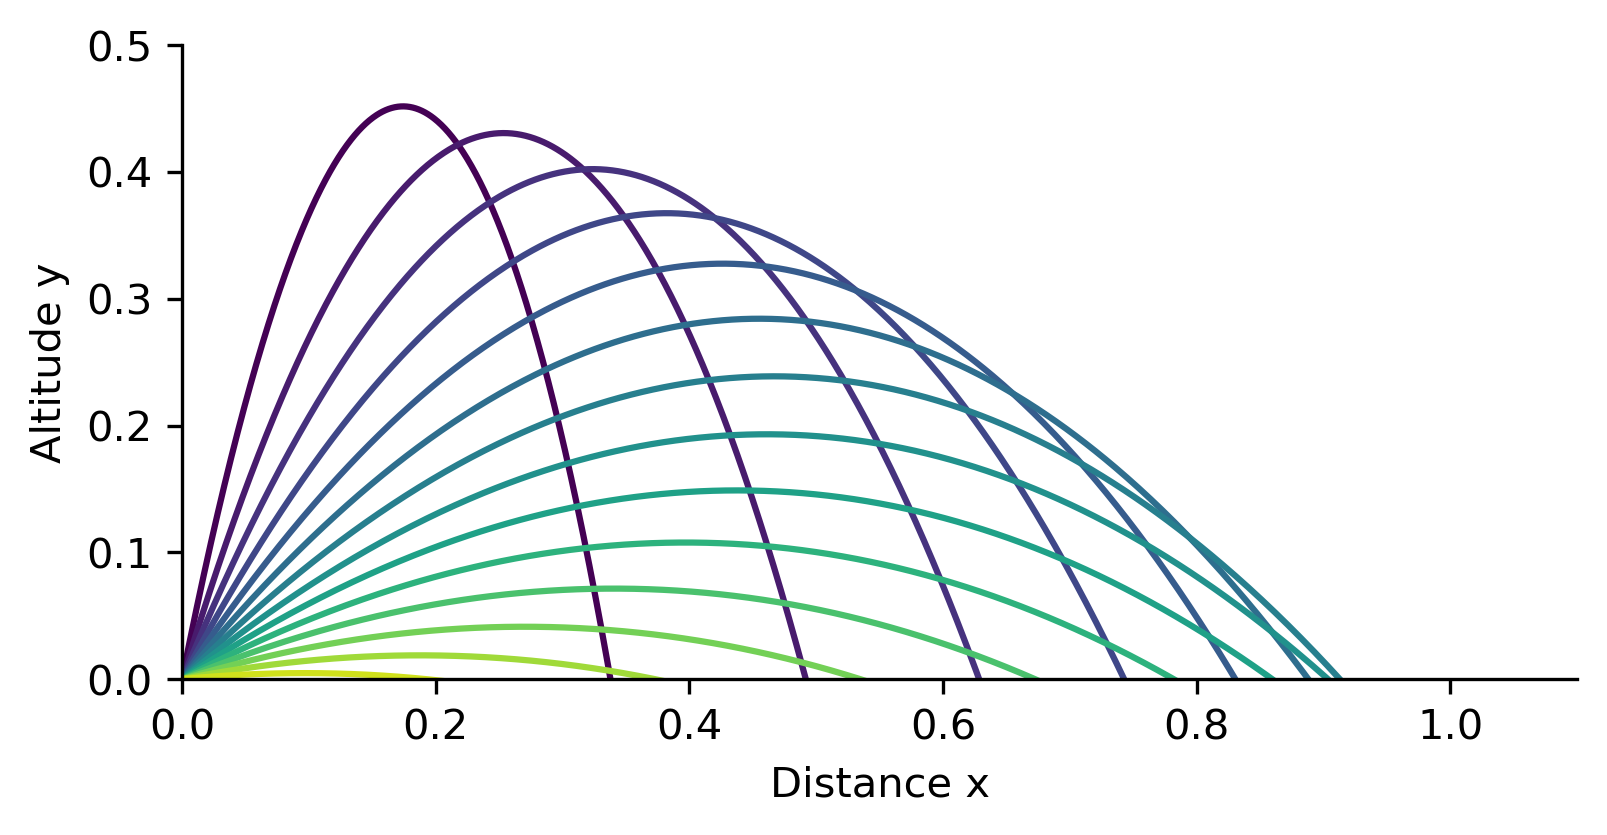
\includegraphics[width=.75\textwidth]{trajectories}
  \caption{
    Trajectoires du projectile pour différentes valeurs de l'angle de hausse.
    A chaque fois, on suppose $\alpha = 0.1$.
    }\label{fig: trajectories}
\end{figure}

\begin{figure}
  \centering
  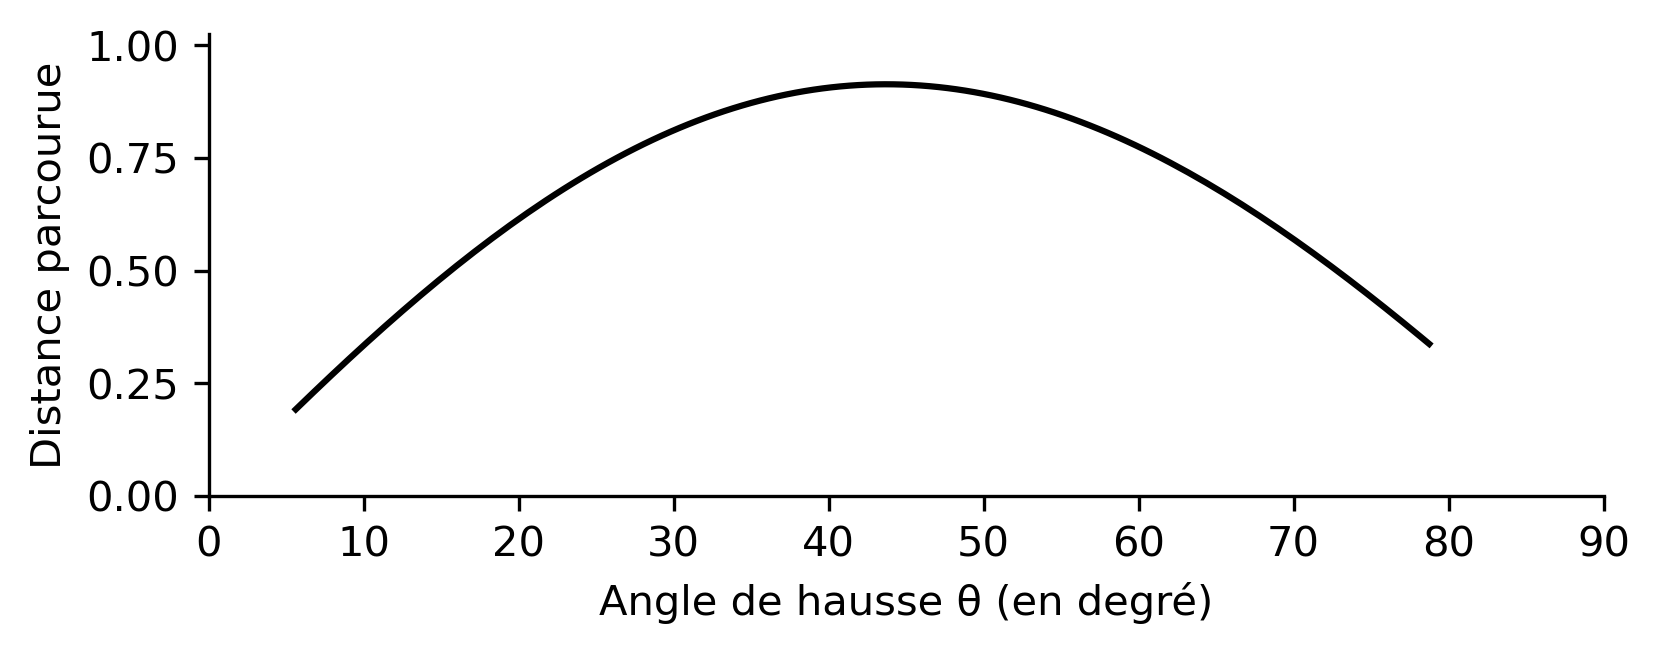
\includegraphics[width=.75\textwidth]{distance_parcourue}
  \caption{
    Distance parcourue par le projectile en fonction de l'angle de hausse du canon.
    On suppose $\alpha = 0.1$.
    }\label{fig: distance parcourue}
\end{figure}
\end{document}
